\section{Gesellschaft}\label{sec:society}

Der gesellschaftliche Einfluss auf die Nachhaltigkeit des Anstiegs der
prognostizierten Tantalproduktion ist global Verteilt. Im Rahmen dieser Analyse
wird der Schwerpunkt auf die wichtigsten Herkunftsländer für die
Tantalproduktion relevanten Mineralien gelegt.

\begin{figure}[h]
    \centering
    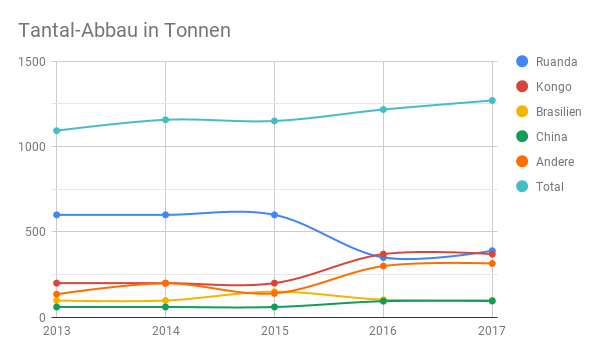
\includegraphics[width=0.8\textwidth]{tantal-abbau_in_tonnen}
    \caption{Weltweiter Tantal-Abbau mit den Top-4 Herkunftsländern. Quelle U.S. Geological Survey ~\cite{USGSMine8}}
    \label{}
\end{figure}

\subsection{Indikatoren}

Nachfolgend werden jeweils die einzelnen Indikatoren beschrieben, welche die
Basis für die gesellschaftliche Entwicklung der Nachhaltigkeit bilden.

\paragraph{Soziale Sicherheit}

Unter der sozialen Sicherheit werden Faktoren im Zusammenhang mit der
politischen Situation der Herkunftsländer zusammengefasst. Insbesondere der
Beitrag an die innenpolitische Stabilität des Landes trägt massgeblich zur
gesellschaftlichen Nachhaltigkeit bei.

\paragraph{Gesundheit}

Die Arbeitsverhältnisse in den Produktionsstätten für Tantal und die Folgen
der Umweltverschmutzung resultierend aus der Produktion auf die lokale
Bevölkerung sind die wichtigsten Aspekte für den Indikator Gesundheit.

\paragraph{Solidarität}

Der Indikator zur Solidarität umfasst das Bewusstsein der Konsumenten und
Märkte zur Herkunft und Produktion von Tantal.

\paragraph{Chancengleichheit}

Die Chancengleichheit umfasst das Verhältniss von Arbeitnehmer und
Arbeitnehmer in den Produktionsstätten, sowie den Einfluss auf die lokale
Bevölkerung.

\subsection{Bewertung}

\paragraph{2013} Gemäss dem U.S. Geological Survey stammen über 60\% der Mineralien für die
Tantalproduktion aus Zentralafrika ~\cite{USGSMine8}. Die Hälfte davon
wird in der Demokratischen Republik Kongo abgebaut, welches als eines der ärmsten
Ländern der Welt gilt gemessen am Human Development Index ~\cite{UNDProgramme2018}. Der Abbau von Mineralien im
Kongo wird von den verschiedenen Konfliktparteien kontrolliert, welche wiederum
den Erlös aus den Minen zur Finanzierung des Konflikts nutzen. Aus diesem Grund
wird Tantal als Konfliktmineral klassifiziert ~\cite{doevenspeck2012konfliktmineralien}.
Gesellschaftlich führt dies zu einem negativen Einfluss im Bereich der sozialen
Sicherheit, da ein wesentlicher Teil des Gesamtvolumens aus Konfliktregionen
stammt und so zur destabilisierung der betroffenen Regionen beiträgt. [Insert citation]
Im Bezug auf die Gesundheit wirkt sich die Tantalgewinnung ebenfalls negativ auf, da die 
Produktionssätten in den Konlfiktgebieten ohne Rücksicht auf die Arbeiter und umliegende Umwelt
operieren. [insert citation]

Im Bezug auf den Indikator zur Solidarität kann eine positive Entwicklung vermerkt werden.
Dies zeigt sich an den zunehmenden Bemühungen die Einfuhr von Konfliktmineralien 
aufzudecken und Einhalt zu gebieten. Als Beispiel sagt die EU-Verordnung zu Konfliktmineralien[insert citation], 
welche im Jahr 2017 in Kraft getreten ist, dass alle Tantal-Importe in die EU die Standards zur nachhaltigen Beschaffung, 
definiert durch die OECD, erfüllen müssen ~\cite{europeancommission}. Die Effektivität solcher 
Massnahmen muss sich aber erst zeigen. So gibt es bereits eine Studie von Germanwatch zur EU-Verordnung, 
welche kritisiert, dass "Unternehmen mit Scheinlösungen davonkommen könnten" ~\cite{Governan35}.

In den Konfliktgebieten des Kongo und den Nachbarsländern wie Ruanda ist der Abbau von 
Mineralien zur Produktion von Tantal eine wichtige Einkommensquelle für die lokale Bevölkerung
und eines der Haupt-Exportgüter der jeweiligen Länder [insert citation]. Dies fliesst in
die Bewertung der Chancengleichheit ein, da ohne den Export dieser Mineralien die Verarmung
der Bevölkerung stark ansteigen würde ~\cite{DRCongo35}.

\paragraph{2035 bei anhaltendem Trend} Die Entwicklung der Konfliktregionen über die nächsten 20 Jarhe
ist kaum vorherzusagen. Auf Grund der Tatsache die Demokratische Republik Kongo seit ihrer Unabhängigkeit
in 1960 von Gewaltausbrüchen geprägt ist und die Situation sich zu bessern scheint ~\cite{Demokrat2}, wird für die 
Prognose angenommen, dass sich die Situation in den Konfliktgebieten nicht bedeutend bessern wird.
Die Soziale Sicherheit wird für 2035 daher gleich bewertet wie 2013. 

% todo gesundheit und solidarität

Die Chancengleichheit wird sich im Bezug auf die starke Nachfrage von Tantal vorallem in Ländern wie
Australien verbessern, wo auf Grund mangelnder Rentabilität eine der grössten Tantalminen der Welt ende 2008 
eingestellt wurde [insert citation]. Durch die steigenden Preise werden die Minen wieder rentabel und 
können so der Bevölkerung wieder neue Arbeitsplätze schaffen.  


\paragraph{2035 mit Kondensatorenalternative}


\begin{table}[h]
    \centering
    \begin{tabular}{l|lll} & \textbf{2013} & \textbf{2035} &  \textbf{2035 mit Annahme} 
        \\ \hline Soziale Sicherheit    & 2  & 2  & 2
        \\ Gesundheit                   & 3  & 5  & 5
        \\ Solidarität                  & 6  & 5  & 5
        \\ Chancengleichheit            & 6  & 7  & 3
        \\ \hline \textbf{Endbewertung} & 4  & 5  & 5
    \end{tabular}
\end{table}
